\documentclass[10pt,twocolumn,letterpaper]{article}

\usepackage{cvpr}
\usepackage{times}
\usepackage{epsfig}
\usepackage{graphicx}
\usepackage{amsmath}
\usepackage{amssymb}
\usepackage{caption}
\usepackage{subcaption}
\usepackage{xcolor}

% Include other packages here, before hyperref.

% If you comment hyperref and then uncomment it, you should delete
% egpaper.aux before re-running latex.  (Or just hit 'q' on the first latex
% run, let it finish, and you should be clear).
\usepackage[breaklinks=true,bookmarks=false]{hyperref}

\cvprfinalcopy % *** Uncomment this line for the final submission

\def\cvprPaperID{****} % *** Enter the CVPR Paper ID here
\def\httilde{\mbox{\tt\raisebox{-.5ex}{\symbol{126}}}}

\def\ti{\mathbf{t}_i}
\def\si{\mathbf{s}_i}

\newcommand{\ignore}[1]{}
\DeclareMathOperator*{\argmin}{arg\,min}

\newcommand{\TODO}[1]{
	{\bfseries\colorbox{red}{\color{white}TODO: #1}}
}

% Pages are numbered in submission mode, and unnumbered in camera-ready
%\ifcvprfinal\pagestyle{empty}\fi
\setcounter{page}{1}
\begin{document}

%%%%%%%%% TITLE
\title{Stereo View Synthesis using Patch Match}

\author{Alexandre Kaspar\\
\\
{\tt\small akaspar@csail.mit.edu}
}

\maketitle
%\thispagestyle{empty}

%%%%%%%%% ABSTRACT



\begin{abstract}
We explore image analogies applied to stereoscopic data synthesis by leveraging an external source of stereo data instead of estimating scene motion or using geometric cues to infer depth / disparity.
We present our approach to work with a large database of such images and provide insights on disparity computation given our findings.
\end{abstract}

%%%%%%%%% BODY TEXT


\section{Introduction}

The emergence of novel 3D displays, the advances in 3d modeling as well as computer vision all call for cheap and user-friendly methods to produce stereoscopic images and videos.
Still, capturing stereoscopic videos remains expensive as it requires specific material, a more complicated camera setting, and it cannot be done for already existing monocular videos
Therefore many efforts have been put in synthesizing stereo data from monocular video streams.
However, this process requires tedious work which casual individuals are likely to not undertake.
We therefore propose to leverage the increasing amount of virtual and real stereoscopic data to automatically synthesize stereoscopic images from monocular images.

\subsection{Related work}

The motivation for this experimental work derives from the recent progress in multiple related domains which we present now.

\paragraph{Texture Synthesis}
Texture is important for photorealistic depiction as it provides a succinct description of surface properties and details which can be hard to specify otherwise.
\ignore{
It is extensively used in computer graphics for augmenting coarse geometric models with fine surface details, while imaging softwares such as Photoshop have been using it to provide hole filling, seamless blending and other tools where the impression of detail matters.
}
It was already extensively used in computer graphics for augmenting coarse geometric models with fine surface details, and now imaging softwares such as Photoshop use it to provide hole filling, seamless blending and other tools related to image-based rendering.

Recent non-parametric exemplar-based texture synthesis algorithms have been very successful, enabling many interesting novel image rendering applications.

From Pixel-based~\cite{Efros99, Wei00, Tong02} and Patch-based~\cite{Praun00, Efros01, Liang01, Kwatra03} methods that grow textures using exemplar pixels or patches, to new optimization-based~\cite{Kwatra05, Darabi12} methods, synthesis has become more reliable, controllable and fast~\cite{Ashikhmin01, Matusik05, Lefebvre06, Lu07}.

It has been used in several fields outside of simple image synthesis \cite{Wei09} such as video textures \cite{Schodl00, Schodl02, Agarwala05} and spatio-temporal video texture synthesis \cite{Kwatra03, Wexler07}.

\paragraph{Image Analogies}
One particular domain where synthesis has brought interesting applications is that of texture / style transfer~\cite{Efros01, Hertzmann01}. By using constrained texture synthesis, one can take a reference image mapping and apply it to a new image to produce an \emph{image analogy}. 

\begin{figure}[ht]
	\center
	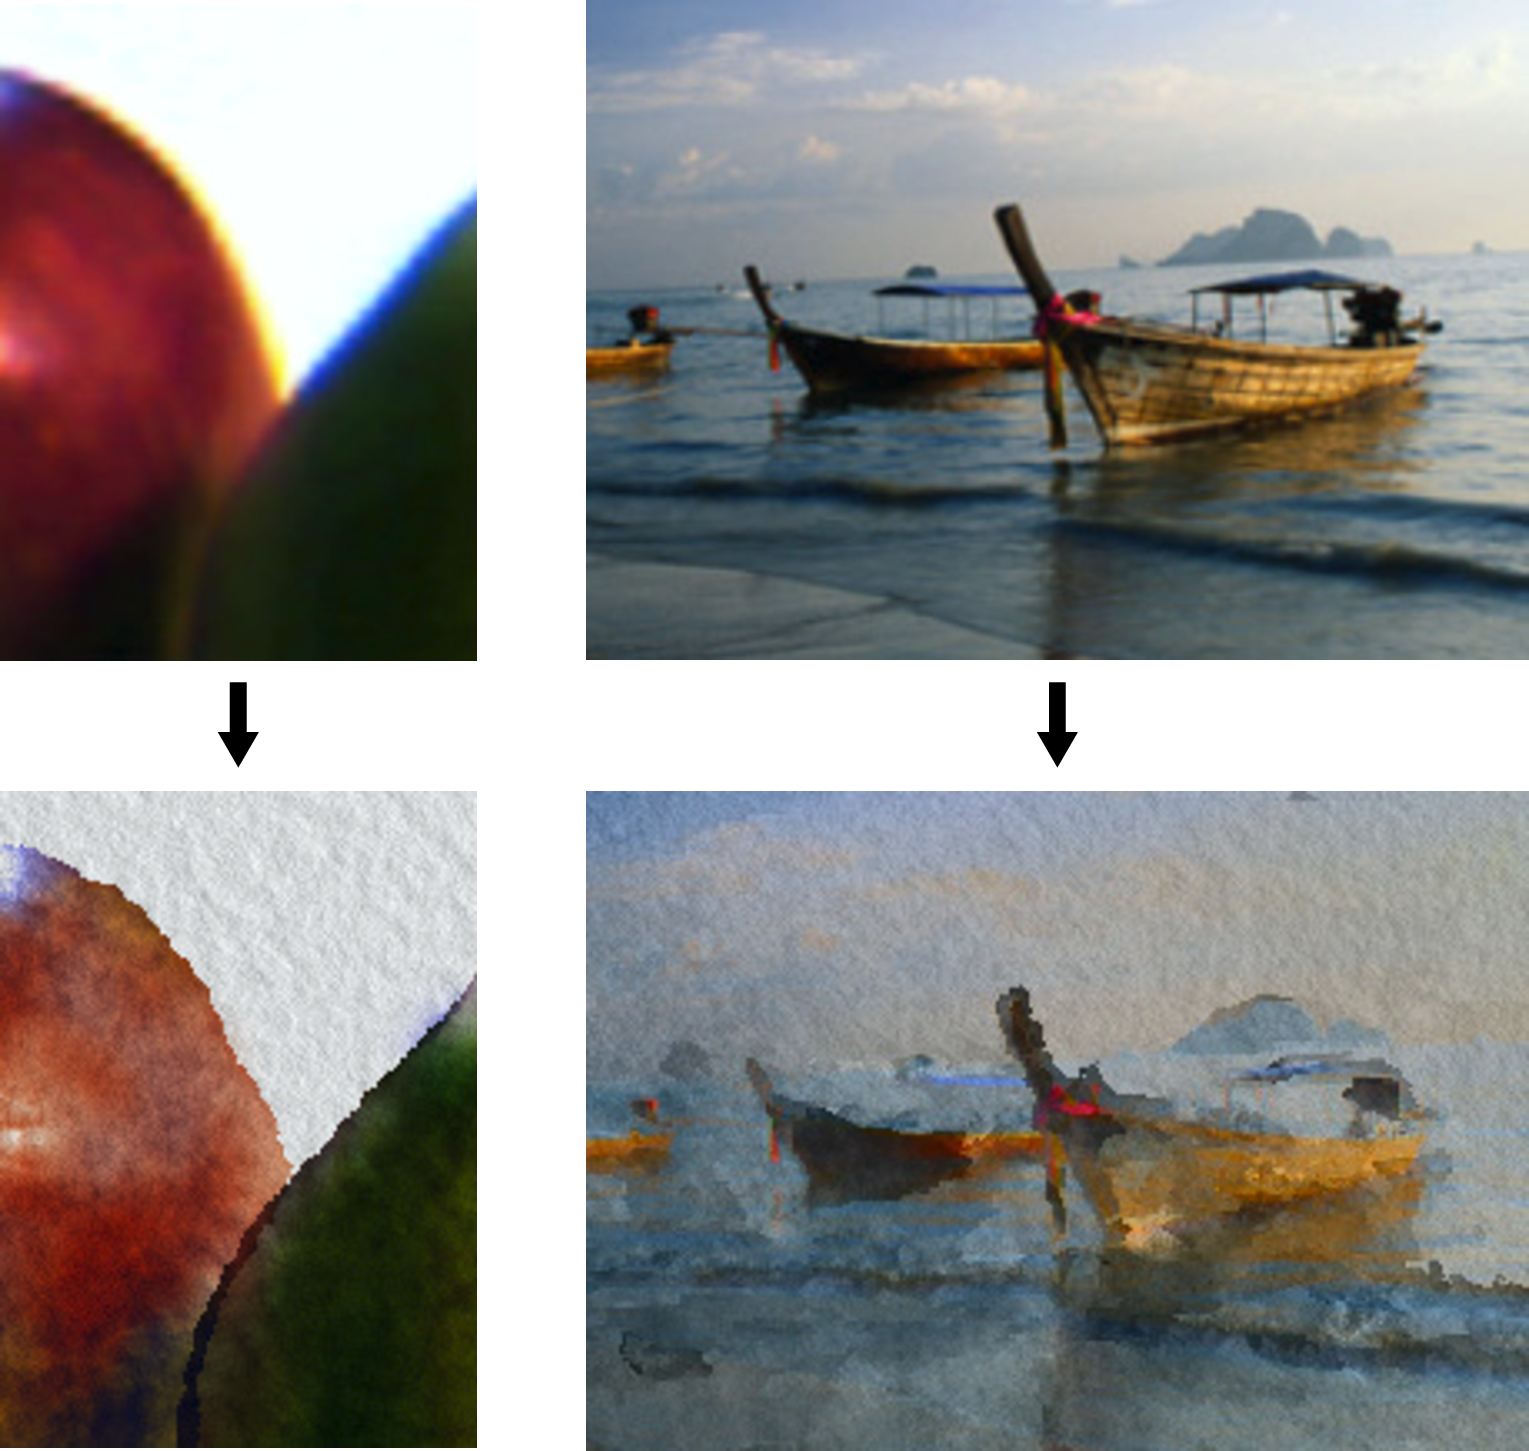
\includegraphics[width=0.45\textwidth]{figures/analogies}
	\caption{Example of image analogy: on the left is the example pair, the top right image is the input, the bottom right one is the analogy output, that transfer the style from the left pair to the image input.}
\end{figure}

\paragraph{Image Querying}
The increasing amount of available images has brought new algorithms for querying and processing it such as GIST and bag-of-features~\cite{Oliva01, Torralba08, Douze09}.
Likewise, synthesis algorithms have led to new patch querying data structures (locality sensitive hashing~\cite{Gionis99}, coherency sensitive hashing~\cite{Korman11} and propagation-assisted kd-trees~\cite{He12}) and algorithms such as Patch Match~\cite{Barnes09}.
We build upon a distributed multi-exemplar of the last one called PatchWeb~\cite{Barnes11}.
Such databases have been used for scene detection and completion \cite{Hays07}.

\paragraph{Synthesizing Stereo}
While stereoscopic data is not yet abundant~\cite{Corrigan10, Smolic10}, 
new large free rendered movies have appeared such as Elephants Dream\footnote{\url{https://orange.blender.org/}}, 
Big Buck Bunny\footnote{\url{http://bbb3d.renderfarming.net/download.html}} or 
Sintel\footnote{\url{https://durian.blender.org/}}, and efforts have been made to produce true stereo data from these for research purposes.
There have been attempts at synthesizing stereo data from monocular streams but they rely on temporal coherence to either deduce motion~\cite{Moustakas05}, use parallax cues~\cite{Zhang07} or eventually require user assistance \cite{Wang11} without leveraging external data sources.
They follow the traditional multi-view image rendering approach that consists in partially modeling the scene such as with Hyper-lapse videos \cite{Kopf14} or stereo reconstruction \cite{Seitz06}.

In this work, we explore the idea of image analogies applied to stereoscopic image rendering and provide a framework to work with future new stereoscopic databases in this context.

\section{Our Approach}

The general idea is to apply image analogies using stereoscopic data to generate new stereoscopic data.
We simply present the ideas here and implementation details are provided in the following section.

The general steps are:
\begin{enumerate}
	\item \textbf{Select} patches in stereo database that match our monocular image patches
	\item \textbf{Transfer} the corresponding stereoscopic data to synthesize the output frame from our input frame
	\item On a \textbf{scale pyramid} to work at different levels of detail
\end{enumerate}

\subsection{Selecting patches}
The selection of pixels or patches from the database corresponds to finding the Nearest Neighbor Field (NNF) between the patches of our new image and those of our database.

Brute-force computation is not tractable given the quantity of data we are facing.
We chose to implement the PatchWeb algorithm~\cite{Barnes11} that extends Patch Match~\cite{Barnes09} to multiple exemplar NNF computation.

\subsection{Transfering the stereoscopic data}
Having a candidate patch in our database (with its corresponding right/left frame patch\footnote{Without loss of generality, we assume that our input corresponds to a left frame in our database.}), we propose different transfer strategies, namely transferring: the \emph{whole patch}, the \emph{patch difference}, or the \emph{patch disparity} as illustrated in Figure~\ref{fig:transfers}.

\begin{figure*}[ht!]
	\centering
	\begin{subfigure}[b]{0.29\textwidth}
	\centering
		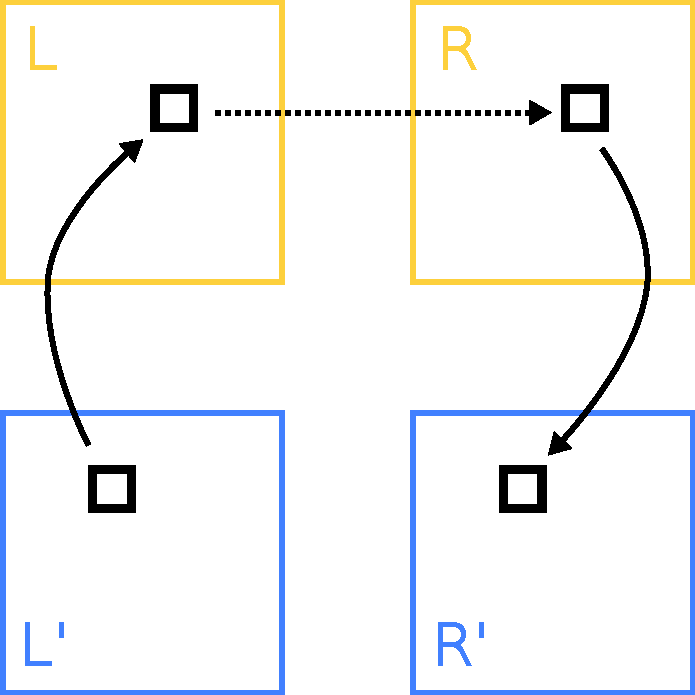
\includegraphics[height=3.6cm]{figures/transfers-A}
		\\
		$L' \to R'=R\phantom{)}$
		\caption{Transferring the whole patch}
	\end{subfigure}
	\begin{subfigure}[b]{0.29\textwidth}
	\centering
		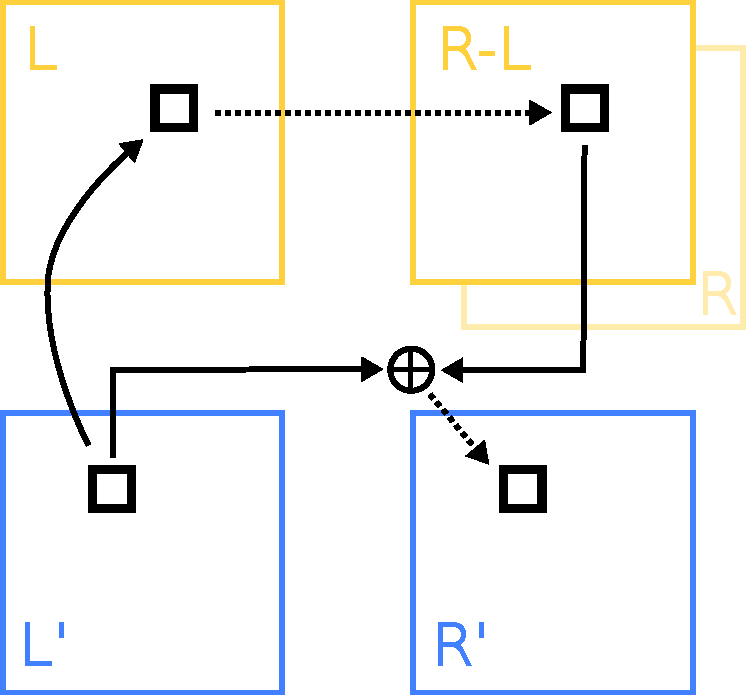
\includegraphics[height=3.6cm]{figures/transfers-B}
		\\
		$L' \to R'=L'+(R-L)$
		\caption{Transferring the patch difference}
	\end{subfigure}
	\begin{subfigure}[b]{0.4\textwidth}
	\centering
		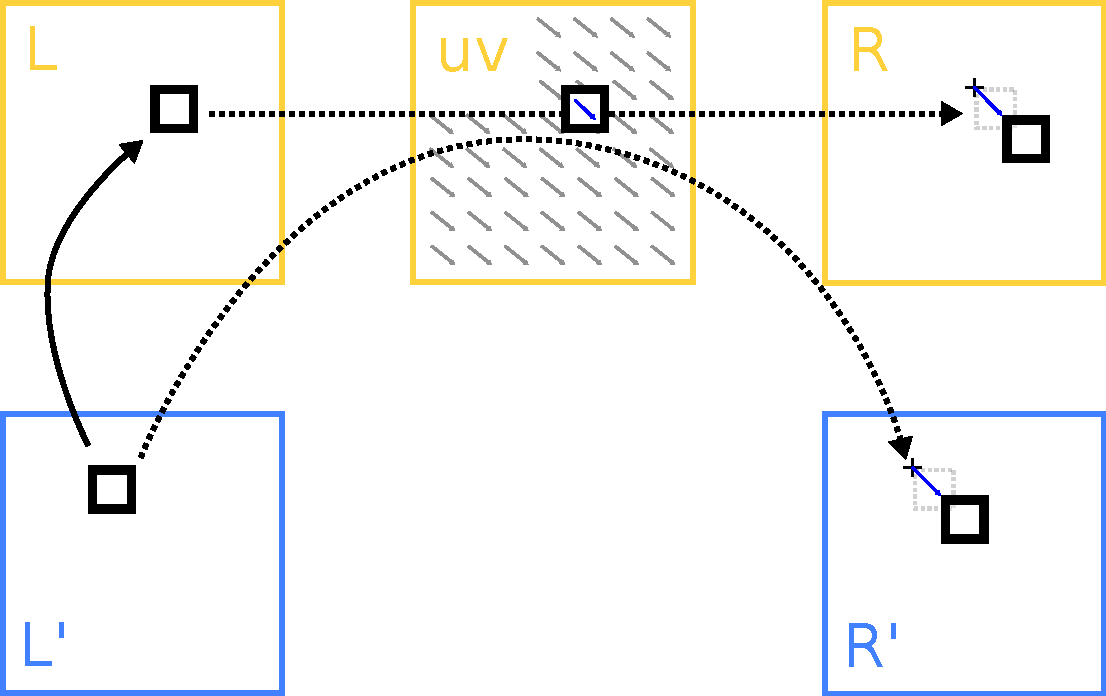
\includegraphics[height=3.6cm]{figures/transfers-C}
		\\
		$L' \to R'=\textrm{warp}_{L\to R}(L')$
		\caption{Transferring the disparity}
	\end{subfigure}
	\caption{Three strategies for stereoscopic data transfer: we synthesize $R'$ from $L'$ given a corresponding mapping $L\to R$}
	\label{fig:transfers}
\end{figure*}

\subsection{Pyramidal processing}
Since different objects and features appear at different scales, we apply the aforementioned selection and transfer on a scale pyramid, in a coarse to fine manner.



\section{Implementation}

We provide details about the nearest neighbor computation with Patch Match~\cite{Barnes09} and its multiple exemplar version Patch Web~\cite{Barnes11}.
Finally, we mention details about the different transfer strategies and especially how we got the frame disparity.

Along this section, we assume that the input frame $L'$ is the left frame and we find a k-NNF from its patches to patches within the left images $L$ of our database.
The database also contains the corresponding right frames $R$ and our goal is to eventually synthesize $R'$ from $L'$.

We assume our images to have $4$ channels: the usual $L+a+b$ from CIELAB that provide perceptually-motivated L2 distances, as well as an extra $y$ channel that encodes the location of pixels within the image, which accounts for disparity being usually larger at the bottom of images than at the top (this helps convergence).
All the channels are normalized to be within $[0;1]$.


\subsection{Patch Match}

Given an input image $A$ made of overlapping $N\times N$ patches $\{\ti\}$, we want to find the closest patches $\{\si\}$ in an image $B$, i.e.
\begin{equation}
	\si^{*} = \argmin_{\si \in B} d(\ti, \si)
\end{equation}
for some distance $d(\cdot)$, usually the sum of squared differences or a L2 norm.

A naive brute-force computation would enumerate all possible patch assignments and find the best one.
However, this is computationally unreasonnable given the context of our large high resolution image database.

Patch Match~\cite{Barnes09} is a fast approximate nearest neighbor algorithm specifically tuned for image patches and thus our problem.
It is based on the \emph{coherence assumption}, namely that, while patches mapped from $A$ to $B$ can be mapped everywhere in $B$, nearby patches in $A$ are usually mapped together in $B$.

\begin{figure}[ht]
\centering
	\begin{subfigure}[t]{0.155\textwidth}
		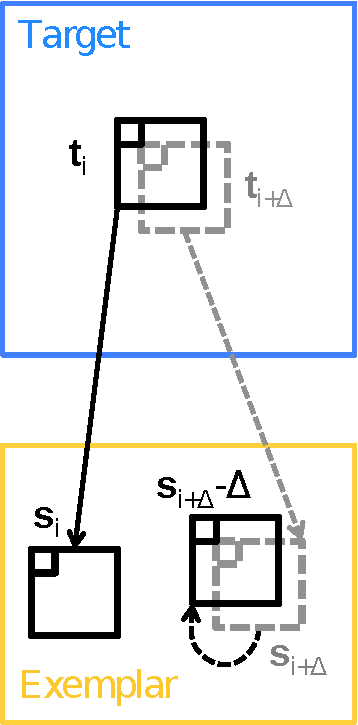
\includegraphics[width=\textwidth]{figures/propagation_text2}
		\caption{Propagation}
	\end{subfigure}
	\begin{subfigure}[t]{0.155\textwidth}
		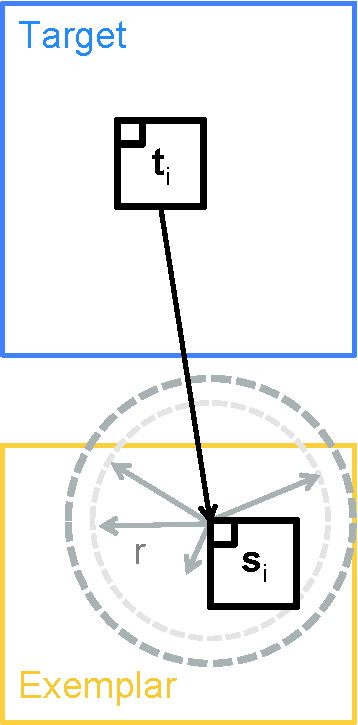
\includegraphics[width=\textwidth]{figures/randsearch_text}
		\caption{Random search}
	\end{subfigure}
	\begin{subfigure}[t]{0.155\textwidth}
		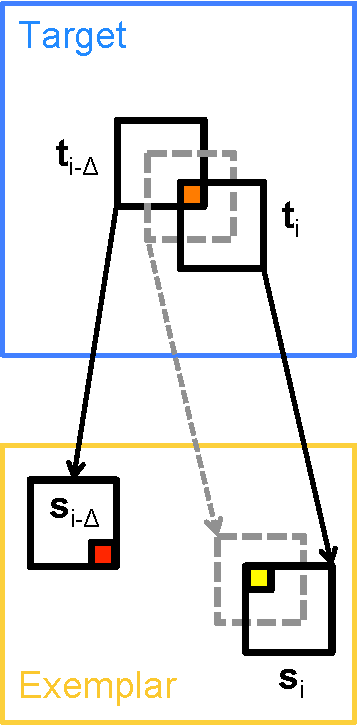
\includegraphics[width=\textwidth]{figures/voting_text}
		\caption{Voting}
	\end{subfigure}
   \caption{The main components of texture synthesis using Patch Match.}
\label{fig:texsynth_patchmatch}
\end{figure}

The algorithm proceeds in scanline-order from an initial guess of the nearest neighbor assignments $\{\ti \to \si\}$ and tries new candidate nearest neighbor patches using two main operations:
\textbf{propagation} which tries to propagate the result of neighboring mappings, and 
\textbf{random search} that randomly samples patches in an exponentially decreasing window (see illustrations in Figure~\ref{fig:texsynth_patchmatch}).

Given these patch assignments, we can transfer localized data.
This last step involves different strategies which we details in Section~\ref{sec:transfer}. 
All of them are forms of \emph{voting} since by having $N\times N$ patches, each of the pixels of our output image technically has as many overlapping patches to choose from.
The usual voting consist of averaging the overlapping pixels which minimizes the average L2 distance.

\paragraph{Extensions}
The Patch Match algorithm has been extended in several ways \cite{Barnes10} including the sampling of rotations, scales and mirrored patch spaces, the use of gain and bias adjustment, a $k$-NN version of the algorithm as well as extra operations (uniform sampling, enrichment and binning).

Application-specific variants of voting have been explored such as Meanshift \cite{Wexler07}, Histogram weighting \cite{Kopf07} as well as Bidirectional Similarity \cite{Simakov08}.

\subsection{Patch Web}
Extending the algorithm to multiple exemplars can seem straightforward: patches now also contain new variable index which represents the exemplar they come from.
However, in practice, dealing with multiple images (and potentially many of them) involves dealing with caching and distributing the computation wisely.

\subsubsection{Additional sampling strategies}
To improve performance, the original algorithm~\cite{Barnes11} makes use of three additional sampling strategies:

\paragraph{Uniform sampling} searches over all patches of all exemplars (this is very similar to random search, with a new exemplar dimension to search through).

\paragraph{Enrichment} finds new candidates by looking at what patches we are mapped to, are mapped to (forward enrichment $f$) or to use the reverse mapping (backward enrichment $f^{-1}$) similarly.
Variants consider multiple hops such as $f^2$, $f^3$, $\dots$ or $f^{-2}$, etc.

Given a $k$-NNF, one can use enrichment with the $k$ candidates or a subset, leading to many potential variants.

\paragraph{Binning} divides the patches into bins similarly as with a histogram, and samples patches from the bin corresponding to the patch we sample for.
To bin patches, usually a lower-dimension space is used ($N\times N$ patches with $C$ channels have $CN^2$ dimensions) by computing PCA.

Recent alternatives~\cite{He12} use Walsh-Hadamard Transform bases~\cite{Hel05} instead of PCA.

Our implementation contains all the aforementioned candidate lookups but binning because of the high memory requirement that makes it harder to implement wisely (other strategies require basically no additional memory storage).
Note that WHT is a better candidate than PCA because it can be computed with much fewer operations (and thus a cache-friendly strategy using it can be envisioned).

\subsubsection{Computing the web}
The general idea is to computer the $k$-NNF from one image in the web to a group of other images and repeat until the web is good enough.
In an ideal world, all images could be loaded at the same time, but given the context of large high resolution images we target, this is not possible.
Instead, we must iteratively do in parallel (for different instances $i$):
\begin{enumerate}
	\item Compute the $k$-NNF from $A_i$ to a subset $\mathbf{A}_i$
	\[ 
		\mathbf{A}_i \subset \bigcup_{j\neq i}{A_j}
	\]
	\item Potentially merge the resulting $k$-NNF with other parallel $k$-NNFs (use minimum distance mappings)
	\item Store/load data on/from disk
	\item Have data caching to compute distances to patches which are not in our current image set\footnote{Otherwise, one must constrain the individual NNFs to always have patches from images in their current lookup set $\mathbf{A}_i$ which is a strong restriction}
\end{enumerate}

\paragraph{Image Subset} we have to eventually process each image once, and to maximize mixing, we start by grouping patches into similar batches, which we compute using GIST features.
Given an image $A_i$ and a budget of $M$ images, for a heterogeneous dataset (not successive similar images), we group $A_i$ with images that have similar GIST descriptors.
We keep a table of the groups and don't process a same group twice since the distance can only get smaller over time.

\paragraph{Convergence} is determined by looking at the number of effective updates done within a $k$-NNF computation.
If no better patch is found for $A_i$, we can short-circuit its scanline processing and go on with other groups.

For a given image, we declare that its $k$-NNF has converged if its best layer (out of the $k$) has distances below some threshold, or a fixed number of iterations has been reached.
The whole algorithm has converged when each individual $k$-NNF has converged.

Since everything is saved to disk, the process can be stopped and resumed later.

\subsection{Stereo Transfer}
\label{sec:transfer}
Armed with an effective multiple exemplar $k$-NNF computation, there remains to transfer the stereoscopic information and synthesize our right frame.

\paragraph{Patch and difference transfer:} we first reduce the $k$-NNF into a single best-layer NNF, and we then use a simple voting strategy with a $7\times 7$ Gaussian mask ($\sigma=1$) for the weight of each overlapping patch so as to reduce blurring.

\paragraph{Disparity transfer:} we transfer it by simply warping our left image $L'$ according to the disparity between $L$ and $R$..

To compute the disparity of each database pair, we used Classic-NL~\cite{Deqing10} for which a fast and simple Matlab/C++ implementation exists.
We also tried to implement our own disparity computation using Patch Match and it turned out to have a higher resolution. However some results were too noisy to be useful.

\paragraph{Disparity computation with Patch Match} several Patch Match-based methods have appeared in the Middlebury evaluations~\cite{Scharstein02}, with a generally fast runtime and good error evaluations~\cite{Bleyer11, Heise13, Jiangbo13, Besse14}.
Extending our Patch Match implementation to compute disparity is simple, we simply modified our set of candidate proposals with:
\begin{itemize}
	\item \emph{Uniform Horizontal Sampling}: uniform sampling with a horizontal constraint
	\item \emph{Random Horizontal Sampling}: random sampling with a decreasing window, and a horizontal constraint
	\item \emph{Propagation}: as usual (we allow vertical deviation by only a few pixels)
	\item \emph{Random Propagation}: propagates the disparity from a uniformly sampled patch
	\item \emph{Local Mean}: uses the weighted average of samples around the current patch (considering only the one-ring neighborhood gives the best results)
\end{itemize}

Furthermore, we vote the disparity by constraining the maximum motion to the 97.5 percentile of disparities within the resulting image (to remove spurious noise).
While such method is not as smooth and doesn't compare to state-of-the-art disparity computations, it produces higher resolution disparity maps than Classic-NL, for an acceptable running time (only a few tens of seconds for mega-pixel images using a $k$-NNF with $k=7$).


\section{Results}

To evaluate our results, we separated a subset of $13$ frames from the two movies Big Buck Bunny and Elephant Dreams and queried another subset of $100$ disjoint frames (all more than $10$ seconds apart from the queries) as our database.
Our database images have a resolution of $960\times 528$ pixels. We used full resolution for query and half resolution ($480\times 264$) for synthesis.

\newcommand{\SA}[3]{\texttt{#1}\texttt{#2}\texttt{#3}}

We tried $12$ different versions of our algorithm given three parameters:
\begin{itemize}
	\item Transfer type: \texttt{P}atch, \texttt{D}ifference or \texttt{F}low (disparity)
	\item Pyramid type: \texttt{G}aussian or \texttt{L}aplacian
	\item Incremental mode: whether to build incrementally (using the $k$-NNF of the previous scale to initialize the next scale) or not
\end{itemize}

A quantitative evaluation is provided in Table~\ref{tbl:results} showing mean squared error with the true right image.
While most results are still far from perfect, they are all better than using the left frame as is (except for one case).
Furthermore they do not provide a qualitative measurement which would in fact be more useful as it has been shown~\cite{Sawhney01, Stelmach00} that stereo frames needn't be high resolution or very close to ground truth to be acceptable.
The human perception takes care of mixing stereoscopic frames and having one bad frame may often not be perceptible (or at least much less than it appears when looking at the isolated bad frame).
We show a few results synthesis in Figure~\ref{fig:stereo_results} to show that a qualitative measurement would be preferable.

As for our own patch-based disparity computation, we show comparisons with Classic-NL-Fast which we used for disparity transfer in Figure~\ref{fig:disp_results}.
\definecolor{goodcolor}{HTML}{009638}
\newcommand{\best}[1]{\underline{#1}}
\newcommand{\good}{\color{goodcolor}}
\newcommand{\bad}{\color{red}}

\begin{table*}
	\centering
	\begin{tabular}{lc|c|cc|cc|cc}
Query & Incr & Left & PG & PL & DG & DL & FG & FL\\\hline
bbb0004 & yes & \best{448.47} & 508.39 & 909.09 & 544.70 & 448.60 & 953.18 & 1167.54 \\
 & no & 448.47 & \good \best{330.71} & 783.08 & \good 473.32 & \good 396.22 & 1001.61 & 1068.16 \\\hline
bbb0058 & yes & 426.54 & \good \best{374.43} & 924.03 & 463.75 & 434.48 & 547.73 & 1316.34 \\
 & no & 426.54 & \good \best{330.07} & 782.21 & \good 416.11 & \good 385.33 & 552.99 & 942.46 \\\hline
bbb0092 & yes & 234.75 & 1493.95 & 509.31 & 305.32 & \good \best{183.69} & 324.44 & 660.46 \\
 & no & 234.75 & \good \best{34.34} & \good 182.56 & \good 47.63 & \good 39.52 & 355.77 & 565.25 \\\hline
bbb0124 & yes & 274.84 & 723.79 & 513.06 & 336.91 & \good  \best{236.69} & 308.30 & 616.81 \\
 & no & 274.84 & \good 67.53 & 448.19 & \good 58.64 & \good \best{51.76} & 294.03 & 568.68 \\\hline
bbb0244 & yes & 858.75 & \good \best{795.20} & 1361.74 & 889.92 & 847.25 & 872.70 & 864.40 \\
 & no & 858.75 & \good \best{703.07} & 1212.19 & \good 845.80 & \good 771.82 & 889.23 & 861.11 \\\hline
bbb0353 & yes & \best{250.49} & 584.98 & 834.15 & 326.76 & 266.40 & 563.66 & 451.24 \\
 & no & \best{250.49} & 314.41 & 677.53 & 313.59 & 254.26 & 542.74 & 423.58 \\\hline
ed0097 & yes & 1649.53 & \good 1130.75 & \good 1132.67 & \good 1646.63 & \good 1565.03 & \good \best{997.70} & \good 1166.23 \\
 & no & 1649.53 & \good \best{1000.37} & \good 1068.22 & \good 1323.11 & \good 1276.36 & \good 1189.43 & \good 1185.89 \\\hline
ed0282 & yes & 175.00 & \good 167.14 & 337.87 & 181.94 & \good 151.15 & \good 156.09 & \good \best{133.29} \\
 & no & 175.00 & \good 165.30 & 306.47 & \good 173.29 & \good 148.44 & 182.94 & \good \best{123.91} \\\hline
ed0438 & yes & 530.54 & \good 347.67 & \good 508.14 & \good 452.37 & \good 410.18 & \good \best{328.59} & \good 349.03 \\
 & no & 530.54 & \good 375.45 & 540.88 & \good 415.17 & \good 358.42 & \good \best{263.60} & \good 324.05 \\\hline
ed0528 & yes & 773.82 & \good 741.03 & \good 681.75 & \good 754.21 & \good 684.74 & \good \best{405.25} & \good 468.93 \\
 & no & 773.82 & \good 513.52 & \good 645.62 & \good 644.25 & \good 579.40 & \good 536.45 & \good \best{449.51} \\\hline
	\end{tabular}
	\caption{Quantitative evaluation of our synthesized frames with the various strategies, the values corresponds to average pixel squared error in $RGB \in [0;255]^3$ space. The first value column includes the error using the left frame as right frame for reference.}
	\label{tbl:results}
\end{table*}

\begin{figure*}
	\centering
	\begin{subfigure}[t]{0.135\textwidth}
		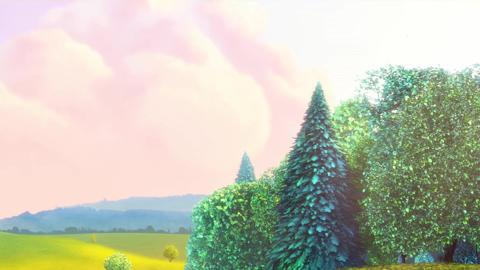
\includegraphics[width=\textwidth]{figures/stereo/bbb_frame-0004-0}\\
		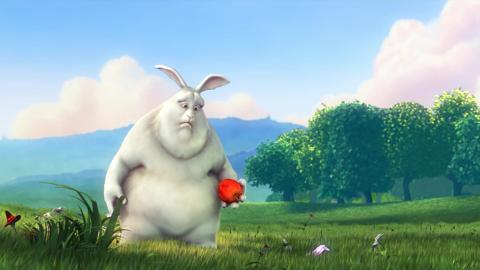
\includegraphics[width=\textwidth]{figures/stereo/bbb_frame-0092-0}
		\caption{Ground truth}
	\end{subfigure}
	\begin{subfigure}[t]{0.135\textwidth}
		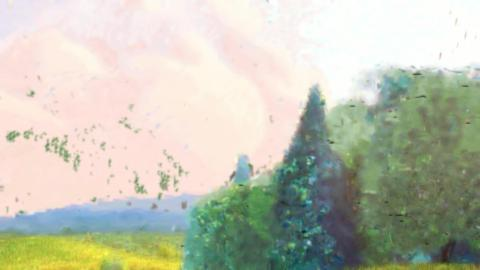
\includegraphics[width=\textwidth]{figures/stereo/bbb_frame-0004-3}\\
		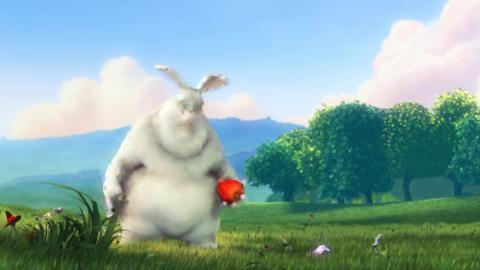
\includegraphics[width=\textwidth]{figures/stereo/bbb_frame-0092-3}
		\caption{PG}
	\end{subfigure}
	\begin{subfigure}[t]{0.135\textwidth}
		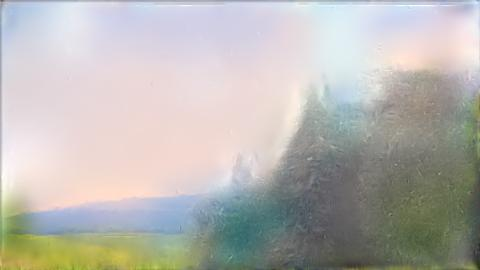
\includegraphics[width=\textwidth]{figures/stereo/bbb_frame-0004-4}\\
		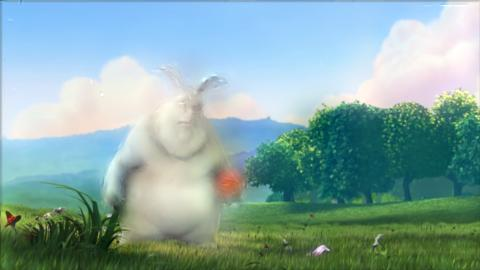
\includegraphics[width=\textwidth]{figures/stereo/bbb_frame-0092-4}
		\caption{PL}
	\end{subfigure}
	\begin{subfigure}[t]{0.135\textwidth}
		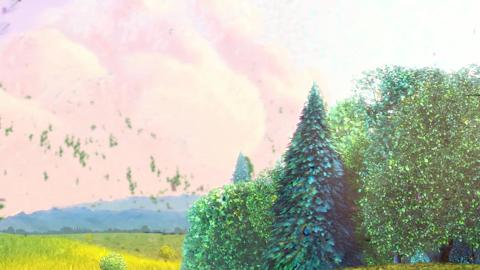
\includegraphics[width=\textwidth]{figures/stereo/bbb_frame-0004-7}\\
		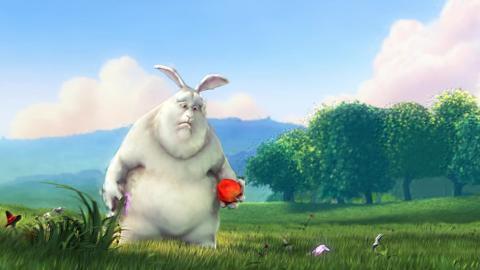
\includegraphics[width=\textwidth]{figures/stereo/bbb_frame-0092-7}
		\caption{DG}
	\end{subfigure}
	\begin{subfigure}[t]{0.135\textwidth}
		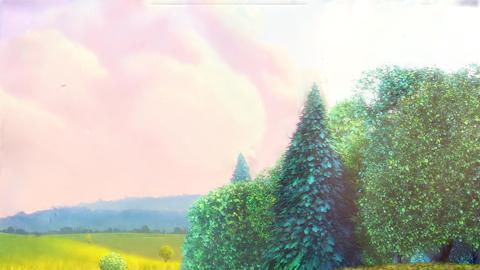
\includegraphics[width=\textwidth]{figures/stereo/bbb_frame-0004-8}\\
		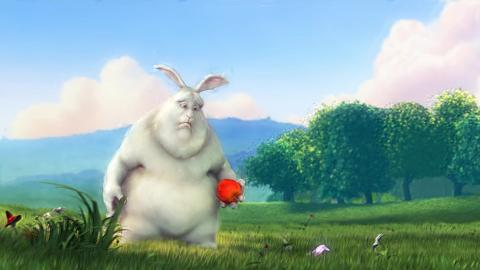
\includegraphics[width=\textwidth]{figures/stereo/bbb_frame-0092-8}
		\caption{DL}
	\end{subfigure}
	\begin{subfigure}[t]{0.135\textwidth}
		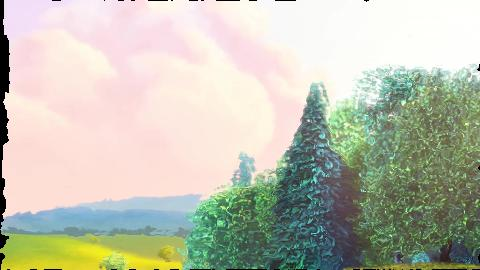
\includegraphics[width=\textwidth]{figures/stereo/bbb_frame-0004-11}\\
		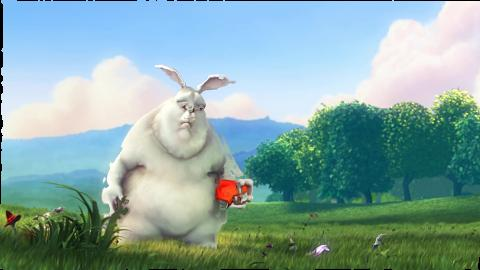
\includegraphics[width=\textwidth]{figures/stereo/bbb_frame-0092-11}
		\caption{FG}
	\end{subfigure}
	\begin{subfigure}[t]{0.135\textwidth}
		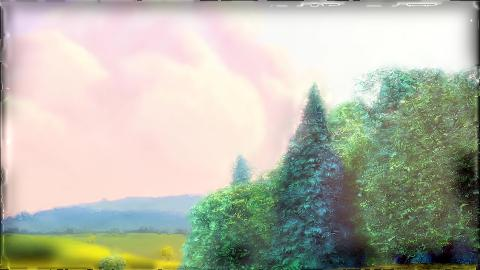
\includegraphics[width=\textwidth]{figures/stereo/bbb_frame-0004-12}\\
		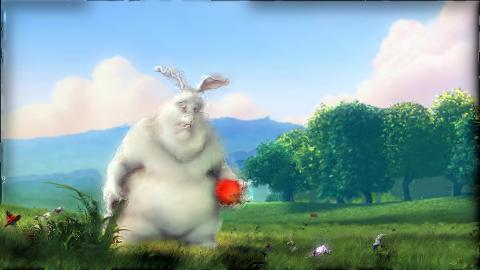
\includegraphics[width=\textwidth]{figures/stereo/bbb_frame-0092-12}
		\caption{FL}
	\end{subfigure}
	\caption{A few examples of stereo analogy results: \texttt{bbb\_frame-0004}}
	\label{fig:stereo_results}
\end{figure*}

\begin{figure*}
	\centering
	\begin{subfigure}[t]{0.24\textwidth}
		
\includegraphics[width=\textwidth]{figures/frames/left/frame-0076}\\
		
\includegraphics[width=\textwidth]{figures/frames/left/frame-0391}
		\caption{Left frame}
	\end{subfigure}
	\begin{subfigure}[t]{0.24\textwidth}
		
\includegraphics[width=\textwidth]{figures/frames/right/frame-0076}\\
		
\includegraphics[width=\textwidth]{figures/frames/right/frame-0391}
		\caption{Right frame}
	\end{subfigure}
	\begin{subfigure}[t]{0.24\textwidth}
		
\includegraphics[width=\textwidth]{figures/classicnlp/frame-0076}\\
		
\includegraphics[width=\textwidth]{figures/classicnlp/frame-0391}
		\caption{Classic-NL-Fast}
	\end{subfigure}
	\begin{subfigure}[t]{0.24\textwidth}
		
\includegraphics[width=\textwidth]{figures/uv/frame-0076}\\
		
\includegraphics[width=\textwidth]{figures/uv/frame-0391}
		\caption{Our patch-based disparity}
	\end{subfigure}
	\caption{A few examples of disparity results}
	\label{fig:disp_results}
\end{figure*}


\section{Conclusion}

The recent synthesis methods we presented produce impressive results from simple and elegant algorithms that require minimum user interaction. The multitude of applications that these methods have brought, as well as the many new potential research problems they generated hopefully show how interesting texture synthesis can be.


{\small
\bibliographystyle{ieee}
\bibliography{report}
}

\end{document}
